% cd ..\..\Users\NikitaSkybytskyi\Desktop\eco-lab
% cls && pdflatex report.tex && cls && pdflatex report.tex && del report.aux, report.toc, report.log, report.out && start report.pdf
\documentclass[12pt, a4paper]{article}
\usepackage[T2A]{fontenc}
\usepackage[utf8]{inputenc}
\usepackage[english,ukrainian]{babel}
\usepackage{amsmath, amssymb}

\usepackage[top = 2 cm, left = 1 cm, right = 1 cm, bottom = 2 cm]{geometry}

\usepackage{float, graphicx}

\usepackage{minted}

\newcommand*\diff{\mathop{}\!\mathrm{d}}

\setlength\parindent{0pt}
\allowdisplaybreaks

\newcommand{\cover}[2]{
\begin{center}
\hfill \break
	Міністерство освіти та науки України \\
	Київський національний університет імені Тараса Шевченка \\ 
	Факультет комп'ютерних наук та кібернетики \\
	Кафедра обчислювальної математики
\end{center}

\vfill 

\begin{center}
	\large{
		Звіт до лабораторної роботи №{#1} на тему: \\ 
		``{#2}'
	}
\end{center}

\vfill 

\begin{flushright}
	Виконав студент групи ОМ-3 \\
	Гронь Ілля
\end{flushright}

\vfill 

\begin{center}
    Київ, 2018 
\end{center}

\thispagestyle{empty} 
\newpage
}

\begin{document}

\cover{1}{Поведінка ізольованої популяції. \\ Модель Леслі вікової структури}

\tableofcontents

\section{Поведінка ізольованої популяції}

Припустимо, що кількість кролів $P(t)$ ($t$ виражається в місяцях) в заповіднику задовольняє диференціальне рівняння \[ \frac{\diff P}{\diff t} = 0.004 \cdot P(t) \cdot (150 - P(t)). \] Нехай спочатку в заповіднику нараховується 50 кролів. Розв'яжіть це диференціальне рівняння та визначте, що станеться з популяцією в майбутньому. \\

Що станеться з популяцією кролів, якщо початкова чисельність тварин становитиме 300 особин? \\

Побудувати графіки чисельності популяцій для двох випадків.

\subsection{Аналітичний розв'язок}

Запишемо обидва питання як задачі Коші для рівняння Бернуллі. \\

Перша задача:
\begin{equation*}
	\left\{
		\begin{aligned}
			& P'(t) = 0.004 \cdot P(t) \cdot (150 - P(t)), \\
			& P(0) = 50.
		\end{aligned}
	\right.
\end{equation*}

Друга задача:
\begin{equation*}
	\left\{
		\begin{aligned}
			& P'(t) = 0.004 \cdot P(t) \cdot (150 - P(t)), \\
			& P(0) = 300.
		\end{aligned}
	\right.
\end{equation*}

Як відомо з курсу диференціальних рівнянь, загальним розв'язком цього рівняння Бернуллі є функція
\begin{equation*}
	P(t) = \frac{150 \cdot e^{0.6 t}}{e^{0.6 t} + C},
\end{equation*}
де стала $C$ визначається початковими умовами. \\

Для першої задачі Коші $C = 2$, і відповідний розв'язок набуває вигляду:
\begin{equation*}
	P(t) = \frac{150 \cdot e^{0.6 t}}{e^{0.6 t} + 2}.
\end{equation*}

Для другої задачі Коші $C = - 0.5$, і відповідний розв'язок набуває вигляду:
\begin{equation*}
	P(t) = \frac{150 \cdot e^{0.6 t}}{e^{0.6 t} - 0.5}.
\end{equation*}

Графіки цих аналітичних розв'язків:
\begin{figure}[H]
	\centering
	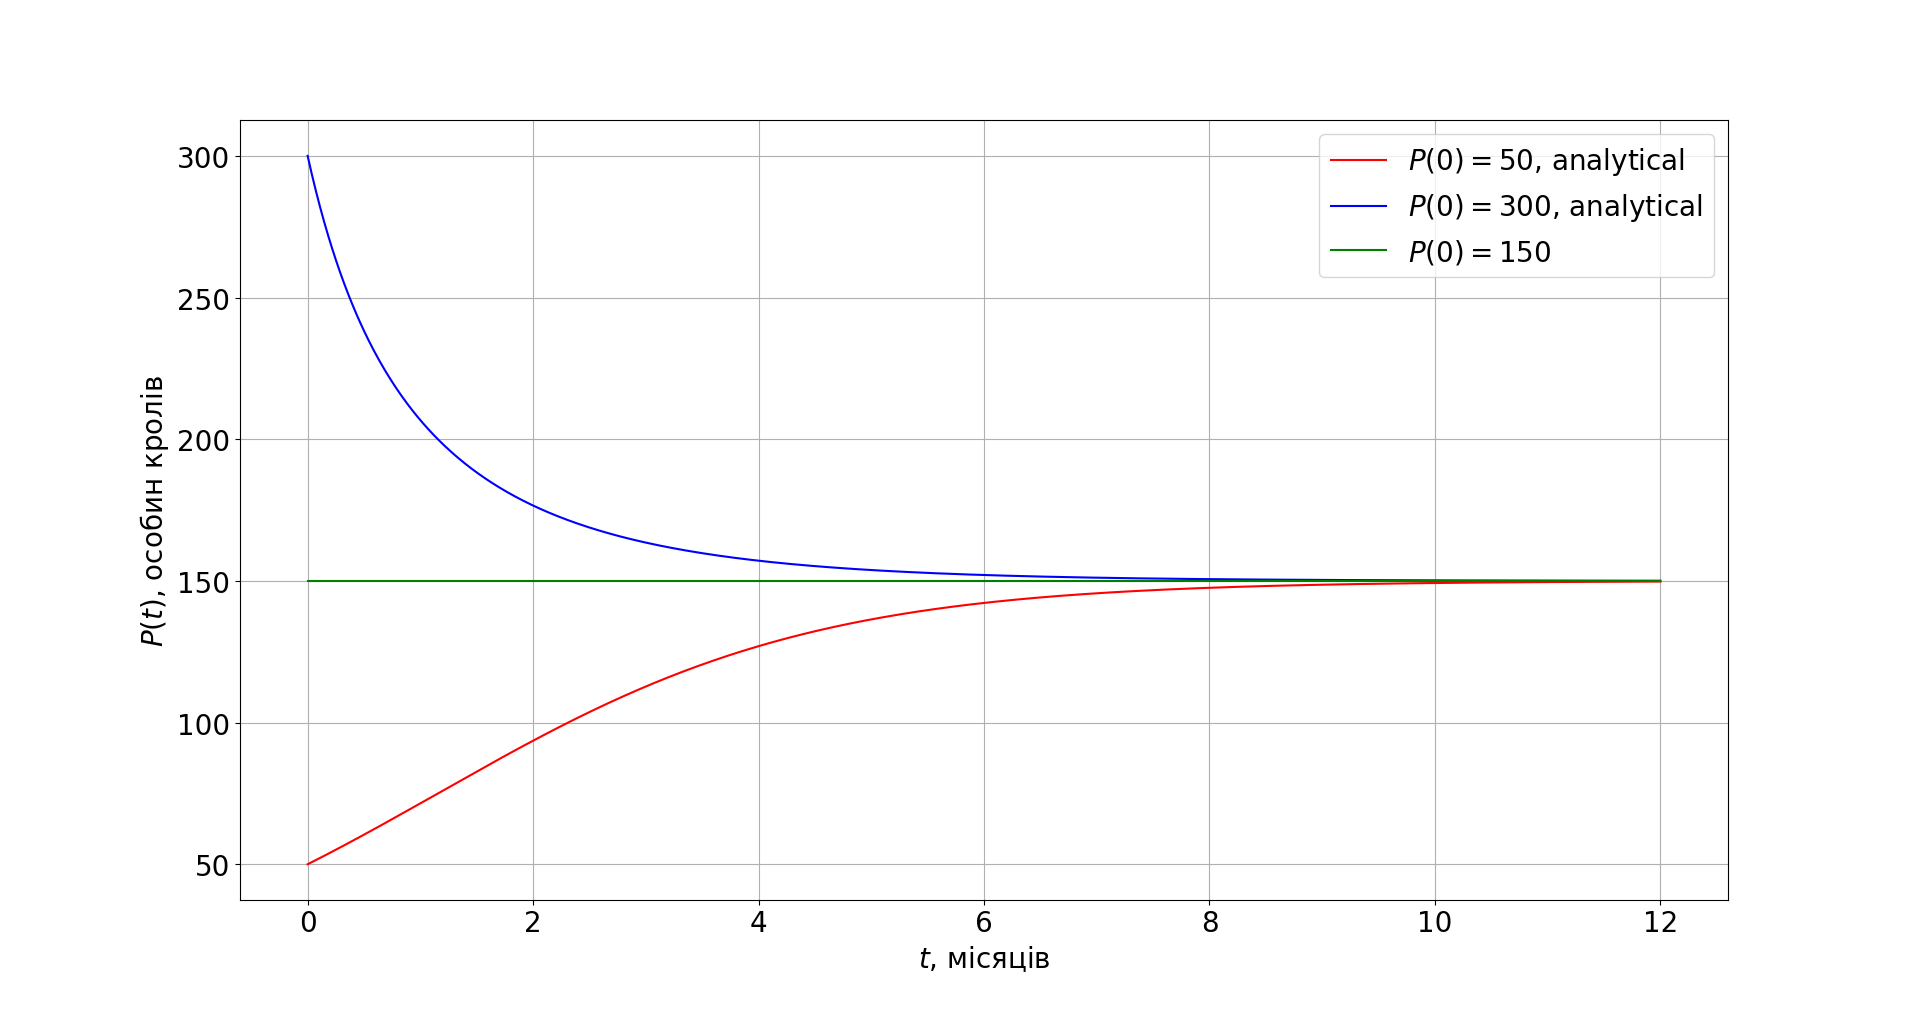
\includegraphics[width=\textwidth]{1_analytical.png}
\end{figure}

\subsection{Чисельне моделювання}

Було використано мову програмування \texttt{Python} і модуль \texttt{scipy.integrate}. Лістинг коду програми:
\inputminted{python}{1_numerical.py}

Графіки отриманих чисельних розв'язків:
\begin{figure}[H]
	\centering
	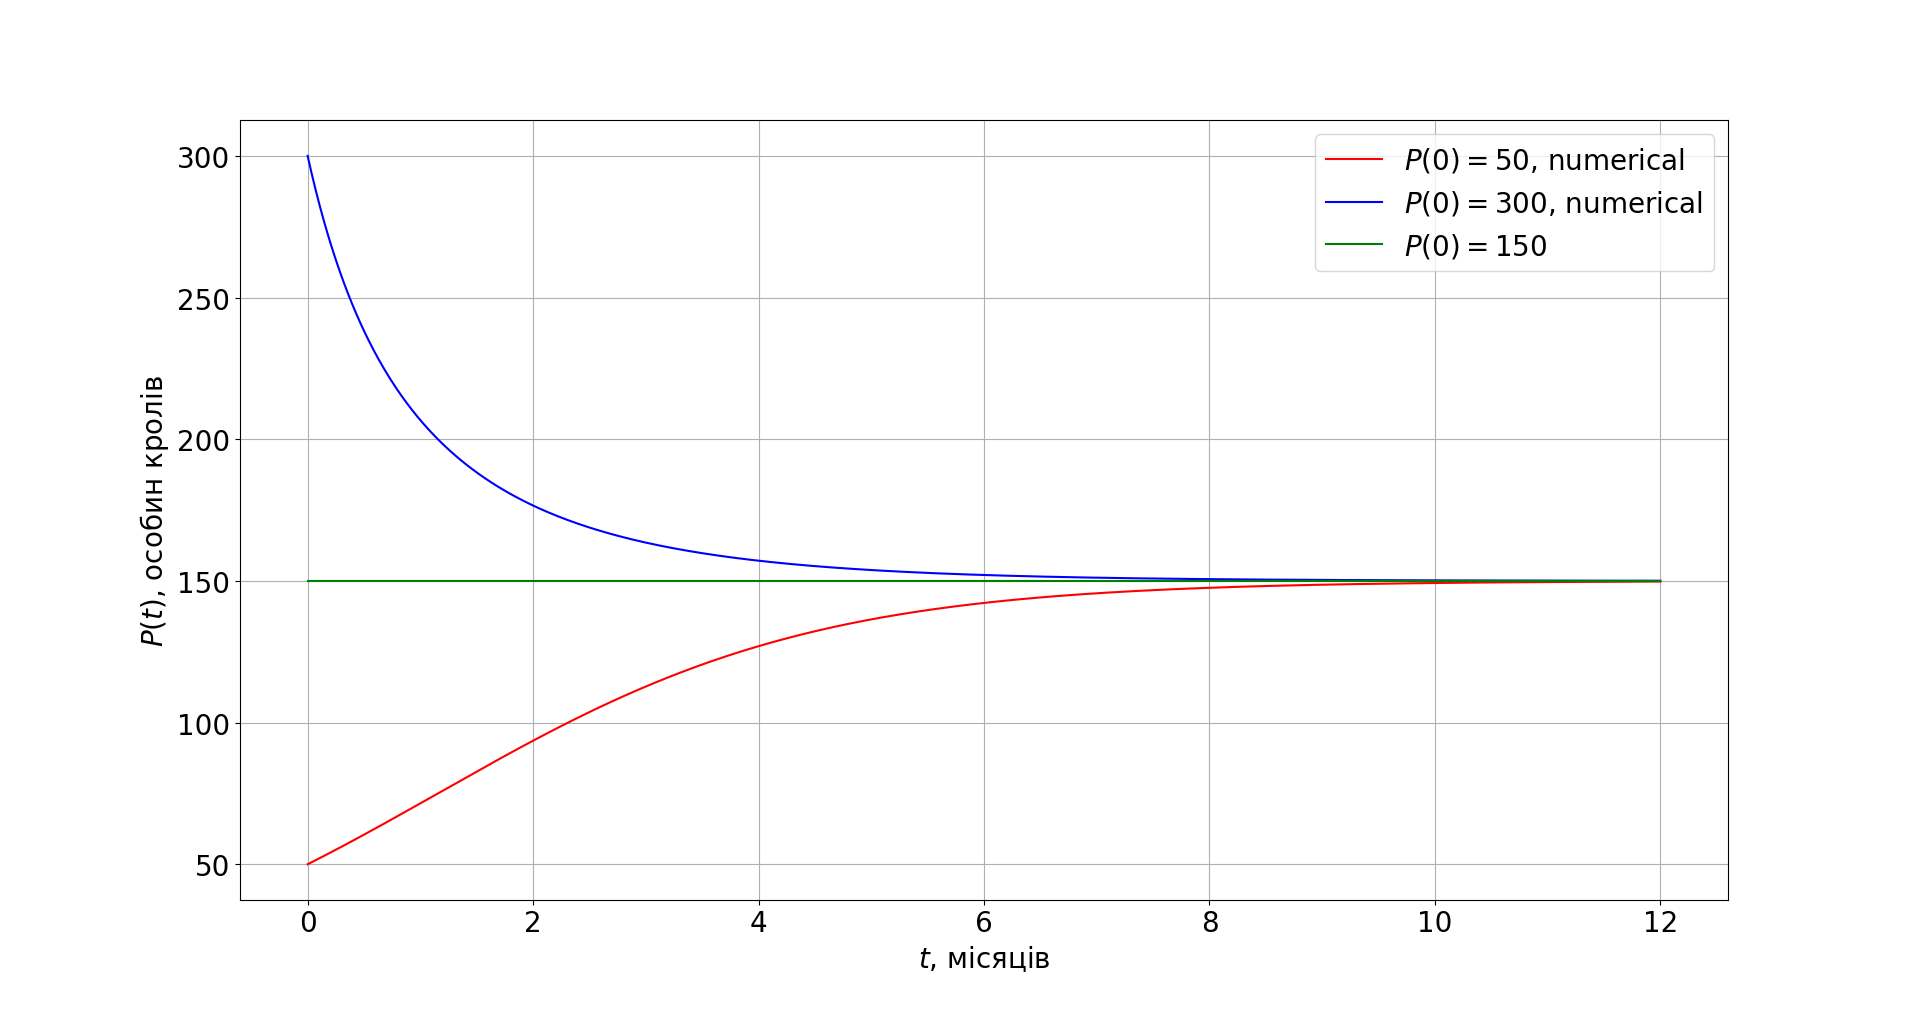
\includegraphics[width=\textwidth]{1_numerical.png}
\end{figure}

Як бачимо отримані графіки (майже) не відрізняються.

\subsection{Висновки про задачу}

Модель що розглядається в задачі -- модель Верхюльста, канонічним записом якої є 
\begin{equation*}
    \frac{\diff N}{\diff t} = r \cdot N \cdot \left( 1 - \frac{N}{q} \right), \quad N(0) = N_0,
\end{equation*}
де $r$ -- коефіцієнт росту. Іншою назвою є ``рівняння логістичного росту''. У нашій задачі коефіцієнт росту -- $150 \cdot 0.004 = 0.6$. \\

Як відомо з теоретичного курсу лекції, модель враховує внутрішньовидову конкуренцію (містить член $-c \cdot N^2$), тому популяції не зростають необмежено а прямують до ємності середовища, у нашому випадку -- 150 особин кролів. \\

Отримані аналітичні та чисельні розв'язки повністю підтверджують теоретичні результати.

\section{Модель Леслі вікової структури}

Вихідна популяція складається з трьох вікових груп. \\

Матриця Леслі має вигляд \[ L = \begin{pmatrix} 0 & 6 & 15 \\ 1/2 & 0 & 0 \\ 0 & 1/2 & 0 \end{pmatrix} \] У початковий момент часу ($t = 0$) популяція складається з однієї самки кожного віку. \\

Знайти:
\begin{enumerate}
	\item склад $x(t)$ у момент часу $t = 5$;
	\item стійку вікову структуру популяції;
	\item момент часу, коли загальна кількість популяції перевищить 75 особин.
\end{enumerate}

\subsection{Чисельне моделювання}

Було використано мову програмування \texttt{Python} і модуль \texttt{numpy.linalg}. Лістинг коду програми:
\inputminted{python}{2.py}

Запишемо $x(t) = L^t \cdot x(0)$, звідси \[ x(5) = L^5 \cdot x(0) = (239.625, 55.125, 16.6875)^T. \]

Для визначення стійкої структури популяції знайдемо власні числа матриці Леслі: \[ \det (L - \lambda E) = \begin{vmatrix} -\lambda & 6 & 15 \\ 1 / 2 & -\lambda & 0 \\ 0 & 1 / 2 & -\lambda \end{vmatrix} = - \lambda^3 + 3 \lambda + \frac{15}{4} = 0. \]

Найбільшим додатним власним числом є \[ \lambda_L = \frac{1}{2} \cdot \left( \frac{1}{3} \sqrt[3]{405 - 27 \sqrt{161}} + \sqrt[3]{15 + \sqrt{161}} \right) \approx 2.17374. \]

Цьому власному числу відповідає власний вектор \begin{align*} x_L &= \left( 8 + \frac{1}{3} \cdot \sqrt[3]{10422 - 810\sqrt{161}} + \sqrt[3]{386 + 30 \sqrt{161}}, \frac{1}{3} \sqrt[3]{405 - 27 \sqrt{161}}+ \sqrt[3]{15 + \sqrt{161}}, 1 \right)^T \approx \\ &\approx (18.9006, 4.34748, 1)^T. \end{align*}

Для зручності пронормуємо цей вектор у $\|\cdot\|_1$-нормі, щоб дізнатися відсоткове співвідношення чисельностей вікових груп, отримаємо \[ \tilde x_L = (0.77946759, 0.17929195, 0.04124046)^T. \]

Як бачимо, у стійкій віковій структурі популяції 78\% особин першої вікової категорії, 18\% особин другої вікової категорії, і 4\% особин третьої вікової категорії. \\

Останнє завдання розв'язуємо простим циклом, ось його вивід:
\begin{table}[H]
	\centering
	\begin{tabular}{|c|c|} \hline
		$t$ & $\|x(t)\|_1$ \\ \hline
		0 & 3 \\ \hline
		1 & 22.0 \\ \hline
		2 & 21.25 \\ \hline
		3 & 77.25 \\ \hline
	\end{tabular}
\end{table}

Як бачимо, чисельність популяції вперше перевищує 75 особин у момент часу $t = 3$.

\end{document}